\documentclass[conference]{IEEEtran}
% \IEEEoverridecommandlockouts
% The preceding line is only needed to identify funding in the first footnote. If that is unneeded, please comment it out.
\usepackage{cite}
\usepackage{amsmath,amssymb,amsfonts}
\usepackage{siunitx}
\usepackage{algorithmic}
\usepackage{graphicx}
\graphicspath{{./images/}}
\usepackage{textcomp}
\usepackage{xcolor}
\usepackage[raggedrightboxes]{ragged2e}
\def\BibTeX{{\rm B\kern-.05em{\sc i\kern-.025em b}\kern-.08em
    T\kern-.1667em\lower.7ex\hbox{E}\kern-.125emX}}
\begin{document}

\title{Pathfinding Robot}

\author{
	\IEEEauthorblockN{James Bao}
	\IEEEauthorblockA{\textit{Dept. of Electrical, Computer,}\\ \textit{and Software Engineering} \\
		\textit{The University of Auckland}\\
		Auckland, New Zealand \\
		jbao577@aucklanduni.ac.nz}
	\and
	\IEEEauthorblockN{Benson Cho}
	\IEEEauthorblockA{\textit{Dept. of Electrical, Computer,}\\ \textit{and Software Engineering} \\
		\textit{The University of Auckland}\\
		Auckland, New Zealand \\
		bcho892@aucklanduni.ac.nz}
	\and
	\IEEEauthorblockN{Nicholas Wolf}
	\IEEEauthorblockA{\textit{Dept. of Electrical, Computer,}\\ \textit{and Software Engineering} \\
		\textit{The University of Auckland}\\
		Auckland, New Zealand \\
		nwol626@aucklanduni.ac.nz}
	\and
	\IEEEauthorblockN{Viktor Neshikj}
	\IEEEauthorblockA{\textit{Dept. of Electrical, Computer,}\\ \textit{and Software Engineering} \\
		\textit{The University of Auckland}\\
		Auckland, New Zealand \\
		vnes637@aucklanduni.ac.nz}
}

\maketitle

\begin{abstract}
	Our Pathfinding Robot is an intelligent, two-wheeled robot capable of navigating the shortest-path between points-of-interest within a maze, projected as a line from a ceiling mounted projector.
	This robot has been developed in COMPSYS 301 during Semester Two of 2023 by Team 1, and has involved the exploration of both hardware and firmware/software aspects.
	This development has included time- and frequency-domain analysis of phototransistor and photodiode sensors, analogue circuit design, sensor constellation \& printed circuit board design, pathfinding algorithm implementation, and firmware development on a PSoC 5LP microcontroller.
	This engineering effort has produced a high-quality, robust robot that comfortably exceeds the goals that we set out to achieve.
	The engineering design considerations and decisions made towards this outcome are outlined in this following report.
\end{abstract}

\begin{IEEEkeywords}
	psoc 5, pathfinding, photodiode, firmware, pcb
\end{IEEEkeywords}



\section{Hardware Design}

\subsection{Frequency Domain Analysis}

% TODO: matlab
% TODO: photodiode vs phototransistor

\subsection{Analogue Circuitry Design}

The goal whilst designing our sensor circuitry was to produce a robust output signal that was immune to ambient lighting conditions.
We concluded in our frequency-domain anayses that this ambient noise primarily consisted of a DC (\qty{0}{\hertz}) component, which could be blocked by a high-pass/coupling capacitor.
Since we decided to use a photodiode, we opted for a transimpedance amplifier instead of a simple resistor due to its lower input/output impedance even when using a feedback resistor in the \unit{\Mohm} range.
The maximum photocurrent for the provided \texttt{SD 019-101-411} photodiode is \qty{2.3}{\uA}, which is very small—hence requiring a large gain.
To get a signal with an acceptable range, where $V_\text{out} = I \times R_\text{feedback}$, we chose a \qty{10}{\Mohm} resistor to produce an output in the order of \qty{2.3}{\volt}.
We also included a feedback capacitor to the transimpedance amplifier that added a low-pass effect, where the cutoff frequency is given by $f_\text{c} = 1 / (2\pi R_\text{feedback}C)$.
Knowing that the relevant projector frequency was \qty{120}{\hertz}, we decided that any $f_\text{c}\geq \qty{300}{\hertz}\sim \qty{400}{\hertz}$ was acceptable, but a higher cutoff would likely be more desirable to minimise any phase-shift effects despite the effect being small.
Consequently, we selected a \qty{40}{\pF} capacitor to produce an $f_\text{c}=\qty{400}{\hertz}$ as it was the smallest capacitor available, and also produced an acceptable $f_\text{c}$.
For the cascaded high-pass stage we decided to choose an $f_\text{c}$ of \qty{110}{\hertz}, assuming the effects of phase shift to be negligible—there was no visible change from experimentation—as this blocks any DC component whilst retaining frequencies of interest.
This also allowed us to select a \qty{42}{\kohm} resistor and a \qty{47}{\uF} capacitor which were readily available in the ECSE Component Store.

The next stage comprised a comparator created with an OpAmp.
No hysteresis was included as we observed our time-domain signals to be very clean with sharp edges.
One disadvantage of this OpAmp topology is that an OpAmp contains an internal capacitor whilst a dedicated comparator IC does not, resulting in a lower slew rate due to the $RC$ time constant.
This was acceptable however as we did not require such precision, and it was more practical to simply use the second OpAmp in the transimpedance amplifier IC.
We decided to use a DAC on the PSoC to provide the comparator reference voltage, as this offered flexibility in case we needed to vary this quantity once our PCB was assembled.

We selected the rail-to-rail \texttt{TLC082} OpAmp as it drove closer to the rails than an \texttt{LM324}, which was essential towards reliably satisfying the high-voltage threshold of the PSoC. We decided against the BJT-based \texttt{LT6221}, as the FET-based \texttt{TLC082} permitted a higher input impedance for each stage due to its lower input bias current (\qty{150}{\nA} for the \texttt{LT6221} versus \qty{50}{\pA} for the \texttt{TLC082}).
In the end, this was prioritised over the slightly higher slew rate of the \texttt{LT6221} (\qty{20}{\volt\per\us}) versus \qty{16}{\volt\per\us}) due to the negligible effects of phase shift in both cases.

\subsection{Printed Circuit Board Design}

% TODO: design considerations
% TODO: constellation

\section{Pathfinding Algorithms}

\subsection{Finding the Shortest Path}

The project requirements state that we must visit five points in \emph{sequential} order, such that the selected algorithm must be capable of computing the shortest path between any two arbitrary points.
Consequently, we decided to explore two different algorithms:
\begin{enumerate}
	\item Dijkstra's Shortest Path (Dijkstra's), and
	\item Breadth First Search (BFS).
\end{enumerate}
Dijkstra's is a greedy algorithm that adds only the least-cost node to its path, whilst BFS is a naïve algorithm—ie the traversal does not have any `intelligence'.
We knew that in this project each point carried no weight, which guaranteed that the first time that BFS saw each node would be the shortest—or shortest equal—path.
It is for this reason that Depth First Search (DFS) was not considered, as it could be proven that DFS is not guaranteed to take the shortest path to an end node, even in an unweighted graph.

We were additionally required to create a tool to demonstrate our implemented algorithms, which we created in \texttt{C++} due to its built-in data structures, whilst retaining a syntax that closely resembled \texttt{C} for easier porting into our firmware.
Additionally, we used \texttt{MatPlotLib} for visualisation.
We verified the functional correctness of both Dijkstra's and BFS with our visualisation tool, but decided to proceed with BFS as it required only a simple queue, whilst Dijkstra's required a priority queue.
As these data structures are not provided in \texttt{C}'s standard library, we elected to reduce the risk of introducing a point of failure by selecting the one with an easier implementation—BFS.

\subsection{Conversion to Instructions}

Finding the shortest path alone would have necessitated a considerable amount of processing and state management in firmware for the robot to remember its position in the maze.
In the interest of simplifying this business logic, we exploit the fact that the pathfinding algorithm only needs to be called at initialisation by implementing a supporting algorithm that generates our required actions, an example of which is shown in Figure \ref{fig:pathfinding-instructions}.

This provides the instructions by which our robot abides at intersections, and specifies the distance for which to travel if the required food location is not found at an intersection.
We verified the correctness of this supplementary algorithm by tracing out the correct path the robot should take and comparing against the generated output.

\section{Firmware Implementation}

In order to facilitate collaboration on different aspects of our firmware, we decided to produce a series of modules, where each module exposed its own API.
This modular architectural approach enabled ease-of-understanding during integration, and prevented name collisions with our use of namespacing.

% TODO: style guide

% TODO: signed magnitude
% TODO: sensor logic design?
% TODO: battery monitoring

\section{Integration}



\section*{Acknowledgment}

A big thank you to our lecturers Dr. Morteza Biglari-Abhari and Dr. Maryam Hemmati; Teaching Assistants Ross Porter, Asher Butler, James Park, and Callum Iddon.

\section*{References}

Coursebook information from COMPSYS 305 directed by Dr. Morteza Biglari-Abhari of the Department of Electrical, Computer, and Software Engineering at The University of Auckland.

\nocite{*}
\bibliographystyle{./IEEEtran}
\bibliography{annot}

\appendix

\begin{figure}[htbp]
	\centerline{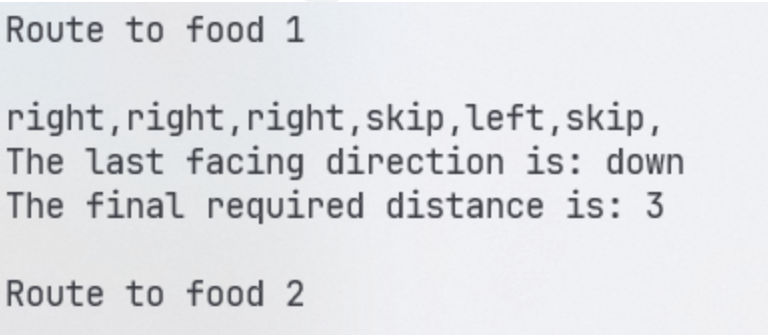
\includegraphics[width=0.5\textwidth]{pathfinding-instructions.png}}
	\caption{Debugging output of the generated instructions}
	\label{fig:pathfinding-instructions}
\end{figure}

\end{document}
